\documentclass[12pt, a4paper]{report}
\usepackage[utf8]{inputenc}
\usepackage[russian]{babel}

\usepackage{graphicx}
\usepackage{listings}
\usepackage{color}

\usepackage{amsmath}
\usepackage{pgfplots}
\usepackage{url}
\usepackage{flowchart}
\usepackage{tikz}
\DeclareGraphicsExtensions{.pdf,.png,.jpg,.svg}
\usetikzlibrary{shapes, arrows}

\usepackage{pgfplotstable}

\renewcommand\contentsname{Содержание}

\usepackage{geometry} 
\geometry{left=3cm} 
\geometry{right=1cm} 
\geometry{top=2cm} 
\geometry{bottom=2cm}

\lstset{ %
language=C++,                 % выбор языка для подсветки (здесь это С)
basicstyle=\small\sffamily, % размер и начертание шрифта для подсветки кода
numbers=left,               % где поставить нумерацию строк (слева\справа)
numberstyle=\tiny,           % размер шрифта для номеров строк
stepnumber=1,                   % размер шага между двумя номерами строк
numbersep=-5pt,                % как далеко отстоят номера строк от         подсвечиваемого кода
backgroundcolor=\color{white}, % цвет фона подсветки - используем         \usepackage{color}
showspaces=false,            % показывать или нет пробелы специальными     отступами
showstringspaces=false,      % показывать или нет пробелы в строках
showtabs=false,             % показывать или нет табуляцию в строках
frame=single,              % рисовать рамку вокруг кода
tabsize=2,                 % размер табуляции по умолчанию равен 2 пробелам
captionpos=t,              % позиция заголовка вверху [t] или внизу [b] 
breaklines=true,           % автоматически переносить строки (да\нет)
breakatwhitespace=false, % переносить строки только если есть пробел
escapeinside={\%*}{*)},   % если нужно добавить комментарии в кодеуказанным 
keywordstyle=\color{blue}\ttfamily,
stringstyle=\color{red}\ttfamily,
commentstyle=\color{green}\ttfamily,
morecomment=[l][\color{magenta}]{\#},
columns=fullflexible }

\usepackage{lipsum}
\setlength{\parindent}{8ex}
\usepackage{indentfirst}

\usepackage{titlesec}
\titleformat{\chapter}[hang]{\LARGE\bfseries}{\thechapter{.} }{0pt}{\LARGE\bfseries}
\titleformat*{\section}{\Large\bfseries}
\titleformat*{\subsection}{\large\bfseries}
 
\begin{document}
 	\begin{titlepage}
 		
 		\begin{center}
 			\Large
 			{\sl Государственное образовательное учреждение высшего профессионального образования\\
 				{\bf«Московский государственный технический университет имени Н.Э. Баумана»\\
 					(МГТУ им. Н.Э. Баумана)}}
 			\noindent\rule{\textwidth}{2pt}
 			\vspace{3cm}
 			
 			{\scshape\LARGE Лабораторная работа №6 \par}
 			\vspace{0.5cm}	
 			{\scshape\LARGE по курсу «Анализ алгоритмов» \par}
 			\vspace{1.5cm}
 			{\huge\bfseries Муравьиный алгоритм \par}
 			\vspace{2cm}
 			\Large Выполнил: Сорокин А.П., гр. ИУ7-52Б\\
 			\vspace{0.5cm}
 			{\Large Преподаватели: Волкова Л.Л., Строганов Ю.В.}
 			
 			\vfill
 			\Large \textit {Москва, 2019 г.}
 			
 		\end{center}
 		
 	\end{titlepage}
 	
 	\tableofcontents
	\newpage
	
	\chapter*{Введение}
	\addcontentsline{toc}{chapter}{Введение}
	
	
	В последние два десятилетия при оптимизации сложных систем исследователи все чаще применяют природные механизмы поиска наилучших решений. Это механизмы обеспечивают эффективную адаптацию флоры и фауны к окружающей среде на протяжении миллионов лет. Сегодня интенсивно разрабатывается научное направление Natural Computing — «Природные вычисления», объединяющее методы с природными механизмами принятия решений, а именно:
	\begin{enumerate}
	\item Genetic Algorithms — генетические алгоритмы;
	\item Evolution Programming — эволюционное программирование;
	\item Neural Network Computing — нейросетевые вычисления;
	\item DNA Computing — ДНК-вычисления;
	\item Cellular Automata — клеточные автоматы;
	\item Ant Colony Algorithms — муравьиные алгоритмы.
	\end{enumerate}

	Эти механизмы обеспечивают эффективную адаптацию флоры и фауны к окружающей среде на протяжении миллионов лет. Имитация самоорганизации муравьиной колонии составляет основу муравьиных алгоритмов оптимизации — нового перспективного метода природных вычислений. Колония муравьев может рассматриваться как многоагентная система, в которой каждый агент (муравей) функционирует автономно по очень простым правилам. В противовес почти примитивному поведению агентов, поведение всей системы получается на удивление разумным.\\
	
	Муравьиные алгоритмы серьезно исследуются европейскими учеными с середины 90х годов. На сегодня уже получены хорошие результаты муравьиной оптимизации таких сложных комбинаторных задач, как: задачи коммивояжера, задачи оптимизации маршрутов грузовиков, задачи раскраски графа, квадратичной задачи о назначениях, оптимизации сетевых графиков, задачи календарного планирования и других. Особенно эффективны муравьиные алгоритмы при online-оптимизации процессов в распределенных нестационарных системах, например трафиков в телекоммуникационных сетях \cite{shtovba}.
	\newpage
	
	\chapter{Аналитическая часть}
	
	В данном разделе будет описан муравьиный алгоритм на примере решения задачи коммивояжера.
	
	\section{Цель и задачи}
	
	Основной целью данной работы является изучение особенностей работы муравьиного алгоритма.
	Для того, чтобы добиться этой цели необходимо выполнить ряд задач:\\
	\begin{enumerate}
		\item примененить знания программирования для реализации муравьиного алгоритма;
		\item получить практические навыки во время выполнения задания;
		\item экспериментально подтвердить различия во временной эффективности работы муравьиного алгоритма при разных значениях коэффицента важности величины пути и коэффициента важности мощности феромона при помощи разработанного программного обеспечения на материале замеров процессорного времени;
		\item описать и обосновать полученные результаты в отчете о выполненной лабораторной работе, выполненном как расчётно-пояснительная записка к работе.
	\end{enumerate}

	\section{Задача коммивояжера}
	
	Задача коммивояжера формулируется как задача поиска минимального по стоимости замкнутого маршрута по всем вершинам без повторений
	на полном взвешенном графе с n вершинами. Вершины графа являются
	городами, которые должен посетить коммивояжер, а веса ребер отражают
	расстояния или стоимости проезда. Эта задача является NP-трудной, и точный переборный алгоритм ее решения имеет факториальную сложность ~\cite{kom}.

	\section{Описание муравьиного алгоритма}
	
	Муравьиные алгоритмы представляют собой вероятностную жадную эвристику, где вероятности устанавливаются, исходя из информации о качестве решения, полученной из предыдущих решений. Идея муравьиного алгоритма - моделирование поведения муравьёв, связанного с их способностью быстро находить кратчайший путь от муравейника к источнику пищи
	и адаптироваться к изменяющимся условиям, находя новый кратчайший
	путь.\\
	
	Моделирование поведения муравьёв связано с распределением феромона на тропе – ребре графа в задаче коммивояжёра. При этом вероятность включения ребра в маршрут отдельного муравья пропорциональна количеству феромона на этом ребре, а количество откладываемого феромона
	пропорционально длине маршрута. Чем короче маршрут, тем больше феромона будет отложено на его рёбрах, следовательно, большее количество муравьёв будет включать его в синтез собственных маршрутов. Моделирование такого подхода, использующего только положительную обратную
	связь, приводит к преждевременной сходимости – большинство муравьёв двигается по локально оптимальному маршруту. Избежать этого можно, моделируя отрицательную обратную связь в виде испарения феромона.\\
	
	C учётом особенностей задачи коммивояжёра, мы можем описать локальные правила поведения муравьёв при выборе пути.
	\begin{enumerate}
		\item Муравьи обладают «памятью». Поскольку каждый город может быть посещён только один раз, то у каждого муравья есть список уже посещённых городов. Обозначим через $J_{i,k}$ список городов, которые необходимо посетить муравью k, находящемуся в городе i.
		
		\item Муравьи обладают «зрением», которое определяет степень желания посетить город j, если муравей находится в городе i. Будем считать, что видимость обратно пропорциональна расстоянию между городами.
		
		\item Муравьи обладают «обонянием», с помощью которого они могут улавливать след феромона, подтверждающий желание посетить город j из города i на основании опыта других муравьёв. Количество феромона на ребре (i,j) в момент времени t обозначим через $\tau_{ij}(t)$.
		
		\item На основании предыдущих утверждений мы можем сформулировать
		вероятностно-пропорциональное правило, определяющее вероятность
		перехода k-ого муравья из города i в город j:

		
		\begin{equation}
		\label{formula_pij}
		P_{ij,k}(t) =
		\begin{cases}
		\frac{(\tau_{ij}(t))^{\alpha}(\eta_{ij}(t))^{\beta}}{\sum\limits_{l \in J(i,k)}(\tau_{il}(t))^{\alpha}(\eta_{il}(t))^{\beta}}, j \in J(i,k)\\
		0, j \notin J(i,k)\\
		\end{cases},
		\end{equation}
		
		где $\tau_{ij}(t)$ – уровень феромона, $\eta_{ij}(t)$ – эвристическое расстояние, а $\alpha$ и $\beta$ – константные параметры.
		
		Выбор города является вероятностным, в общую зону всех городов
		бросается случайное число, которое и определяет выбор муравья. При
		$\alpha$ = 0 алгоритм вырождается до жадного алгоритма, по которому на
		каждом шаге будет выбираться ближайший город.
		\item При прохождении ребра муравей оставляет на нём некоторое количество феромона, которое должно быть связано с оптимальностью сделанного выбора. Пусть есть маршрут, пройденный муравьём k к моменту времени t, Т – длина этого маршрута, $L_{k}(t)$ - цена текущего решения для k-ого муравья а Q – параметр, имеющий значение порядка цены оптимального решения.
		Тогда откладываемое количество феромона
		
		\begin{equation}
		\label{formula_dt}
		\Delta \tau_{ij,k}(t) =
		\begin{cases}
		\frac{Q}{L_{k}(t)}, (i, j) \in T_{k}(t)\\
		0, (i, j) \notin T_{k}(t)\\
		\end{cases},
		\end{equation}
		
		а испаряемое количество феромона
		
		\begin{equation}
		\label{formula_dt}
		\tau_{ij}(t+1) = (1-p)\tau_{ij}(t) + \sum\limits_{k=1}^m \Delta \tau_{ij,k}(t),
		\end{equation}
		
		где m – количество муравьёв в колонии ~\cite{aco}.
	\end{enumerate}
	
	\section{Вариации муравьиного алгоритма}
	
	Ниже приведены вариации муравьиного алгоритма.
	\begin{enumerate}
		
		\item \textbf{Элитарная муравьиная система}.
		Из общего числа муравьёв выделяются так называемые «элитные муравьи». По результатам каждой итерации алгоритма производится усиление лучших маршрутов путём прохода по данным маршрутам элитных муравьёв и, таким образом, увеличение количества феромона на данных маршрутах. В такой системе количество элитных муравьёв является дополнительным параметром, требующим определения. Так, для слишком большого числа элитных муравьёв алгоритм может «застрять» на локальных экстремумах.
		
		\item \textbf{Max-Min муравьиная система}.
		Добавляются граничные условия на количество феромонов ($\tau max$,$\tau min$). Феромоны откладываются только на глобально лучших или лучших в итерации путях. Все рёбра инициализируются значением $\tau max$.
		
		\item \textbf{Ранговая муравьиная система(ASrank)}.
		Все решения ранжируются по степени их пригодности. Количество откладываемых феромонов для каждого решения взвешено так, что более подходящие решения получают больше феромонов, чем менее подходящие.
		
		\item \textbf{Длительная ортогональная колония муравьёв (COAC)}.
		Механизм отложения феромонов COAC позволяет муравьям искать решения совместно и эффективно. Используя ортогональный метод, муравьи в выполнимой области могут исследовать их выбранные области быстро и эффективно, с расширенной способностью глобального поиска и точностью.
	\end{enumerate}

	\section{Вывод}
	
	В данном разделе были изучены различные вариации муравьиного алгоритма.

	\chapter{Конструкторская часть}
	
	В данном разделе в соответствии с описанием алгоритмов, приведенными в аналитической части работы, будет рассмотрена схема муравьиного
	алгоритма.
	
	\section{Схемы алгоритмов}
	
	На рисунке \ref{ris:aco} представлена обобщённая схема муравьиного алгоритма.
	
	\begin{figure}[ht!]
		\centering
		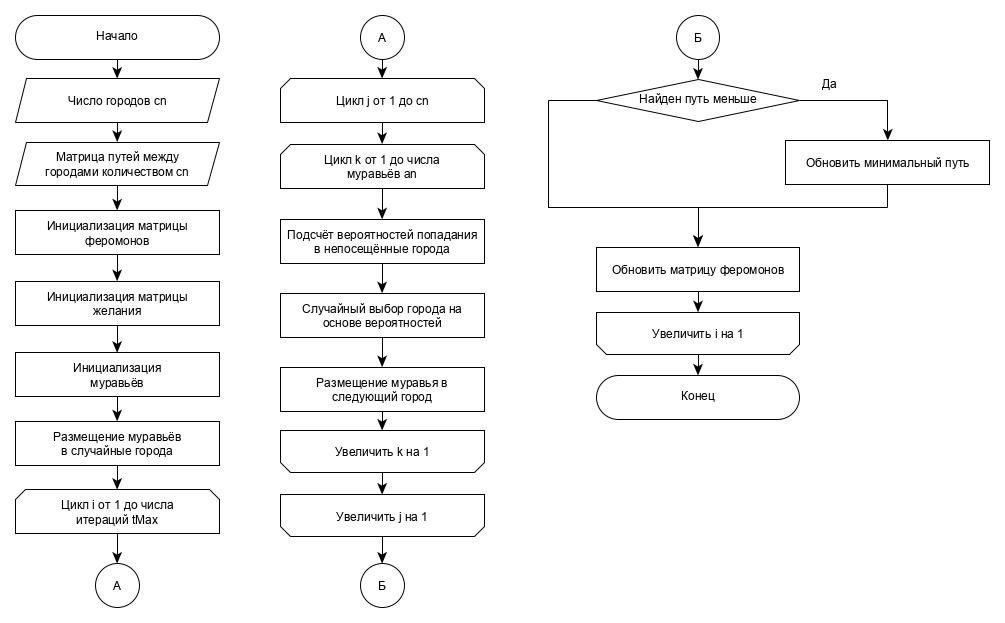
\includegraphics[scale=0.5]{img/aco.jpg}
		\caption{Схема муравьиного алгоритма}
		\label{ris:aco}
	\end{figure}

	\section{Вывод}
	
	В данном разделе были рассмотрены принципы работы и схемы муравьиного алгоритма.
	
    \chapter{Технологическая часть}
    
    В данном разделе приведены требования к программному обеспечению, средствам реализации, а также листинги кода.
    
    \section{Средства реализации}
    
    Для реализации программы был использован язык программирования C++, так как он был подробно изучен в курсе объектно-ориентированного программирования в университете\cite{C}.
    
    Для замера времени использовалась функция, приведенная на листинге\cite{time_b}. Данная функция считает реальное процессорное время в тиках. Для ее работы была подключена библиотека time.h.
   
    \section{Реализация алгоритмов}
    
    В листингах \ref{code_ant_class}, \ref{code_ant_meth}, \ref{code_aco_class}, \ref{code_aco_init} и \ref{code_aco_meth} описана реализация муравьиного алгоритма.
    
    \begin{lstlisting}[label=code_ant_class,caption=Класс муравья Ant]
    class Ant
    {
    public:
    	size_t path_len;
    	std::vector<bool> visited;
    	std::vector<size_t> path;
    
    	Ant(const size_t graph_size);
    
    	void visit_city(const size_t city, const size_t cur_path_len,
    	const size_t cur_path_dist);
    	void clear_visits();
    	void make_default_path();
    	bool is_visited(const size_t city) const;
    };
    \end{lstlisting}
    
    \begin{lstlisting}[label=code_ant_meth,caption=Методы класса Ant]
    Ant::Ant(const size_t graph_size) : path_len(0)
    {
    	for (size_t i = 0; i < graph_size; i++)
    	{
    		path.push_back(0);
    		visited.push_back(false);
    	}
    }
    
    void Ant::visit_city(const size_t city, const size_t cur_path_len,
    	const size_t cur_path_dist)
    {
    	path_len += cur_path_dist;
    	path[cur_path_len] = city;
    	visited[city] = true;
    }
    
    void Ant::clear_visits()
    {
    	for (size_t i = 0; i < visited.size(); i++)
    		visited[i] = false;
    	path_len = 0;
    }
    
    void Ant::make_default_path()
    {
    	path_len = 0;
    	visit_city(path[path.size() - 1], 0, 0);
    }
    
    bool Ant::is_visited(const size_t city) const
    {
    	return visited[city];
    }
    \end{lstlisting}
    
    \begin{lstlisting}[label=code_aco_class,caption=Класс алгоритма ACO]
    class ACO
    {
    private:
    	const std::vector<std::vector<int>> dist_graph;
    	const size_t cities_count;
    
    	std::vector<std::vector<double>> pher_graph;
    	std::vector<std::vector<double>> desire_graph;
    
    	std::vector <Ant> ants;
    	size_t ants_count;
    
    	std::vector<double> paths_probs;
    
    	double alpha = 0.5;
    	double rho = 0.5;
    	size_t tMax = 100;
    	double beta = 1 - alpha;
    
   	 	const double Q = 5;
    	const double ants_factor = 1;
    	const double init_pher_value = 1;
    
    public:
    	size_t min_len = 0;
    	std::vector<size_t> min_path;
    
    	ACO(const Graph<int>& graph);
    
    	void execute();
    	void change_params(double alpha, double rho, size_t tMax);
    
    private:
    	void make_default_state();
	    void init_ants();
	    void init_pher_graph();
	    void pave_ants_paths();
	    size_t get_next_city(const Ant& ant, const size_t cur_city);
	    void update_min_path();
	    void update_pheromones();
	    void make_default_ants();
	    size_t select_next_city();
	    double get_sum_probabilities();
    };
    \end{lstlisting}
    
    \begin{lstlisting}[label=code_aco_init,caption=Методы инициализации и запуск алгоритма]
    ACO::ACO(const Graph<int>& graph) :
    	dist_graph(graph.graph), cities_count(graph.size)
    {
	    // init pher_graph
	    for (size_t i = 0; i < cities_count; i++)
	    {
	    	std::vector<double> line;
	    	for (size_t j = 0; j < cities_count; j++)
	    		line.push_back(init_pher_value);
	    	pher_graph.push_back(line);
	    }
	    
	    // init desire_graph
	    for (size_t i = 0; i < cities_count; i++)
	    {
	    	std::vector<double> line;
	    	for (size_t j = 0; j < cities_count; j++)
	    		line.push_back(dist_graph[i][j] == 0 ? 0 : 
	   				1.0 / dist_graph[i][j]);
	    	desire_graph.push_back(line);
	    }
	    
	    // init ants_count
		ants_count = cities_count * ants_factor;
	    for (size_t i = 0; i < ants_count; i++)
	    {
	    	Ant ant(cities_count);
	    	ants.push_back(ant);
	    }
    
    	// init paths_probs
    	for (size_t i = 0; i < cities_count; i++)
    		paths_probs.push_back(0);
    }
    
    void ACO::execute()
    {
	    make_default_state();
	    init_pher_graph();
	    init_ants();
	    
	    for (size_t i = 0; i < tMax; i++)
	    {
		    pave_ants_paths();
		    update_min_path();
		    update_pheromones();
		    make_default_ants();
	    }
    }
    
    void ACO::change_params(double alpha, double rho, size_t tMax)
    {
	    this->alpha = alpha;
	    this->beta = 1 - alpha;
	    this->rho = rho;
	    this->tMax = tMax;
    }
    
    void ACO::make_default_state()
    {
	    min_len = 0;
	    min_path.clear();
    }
    
    void ACO::init_ants()
    {
	    for (size_t i = 0; i < ants_count; i++)
	    {
	    	ants[i].clear_visits();
	    	ants[i].visit_city(rand() % cities_count, 0, 0);
	    }
    }
    
    void ACO::init_pher_graph()
    {
	    for (size_t i = 0; i < cities_count; i++)
	    	for (size_t j = 0; j < cities_count; j++)
	    		pher_graph[i][j] = init_pher_value;
    }
    \end{lstlisting}
    
    \begin{lstlisting}[label=code_aco_meth,caption=Основные функции муравьиного алгоритма]
    void ACO::pave_ants_paths()
    {
	    for (size_t i = 0; i < cities_count - 1; i++)
	    {
		    for (size_t j = 0; j < ants_count; j++)
		    {
			    const size_t cur_city = ants[j].path[i];
			    const size_t next_city = get_next_city(ants[j], cur_city);
			    const int dist = dist_graph[cur_city][next_city];
			    
			    ants[j].visit_city(next_city, i + 1, dist);
		    }
	    }
	    
	    for (size_t j = 0; j < ants_count; j++)
	    {
		    size_t i_ind = ants[j].path[ants[j].path.size() - 1];
		    size_t j_ind = ants[j].path[0];
		    const int dist_init_city = dist_graph[i_ind][j_ind];
		    ants[j].path_len += dist_init_city;
	    }
    }
    
    size_t ACO::get_next_city(const Ant& ant, const size_t cur_city)
    {
	    double sumP = 0;
	    
	    for (size_t i = 0; i < cities_count; i++)
	    {
	    	double pher_factor = pow(pher_graph[cur_city][i], alpha);
	    	double desire_factor = pow(desire_graph[cur_city][i], beta);
	    	sumP += pher_factor * desire_factor;
    	}
    
    	for (size_t i = 0; i < cities_count; i++)
    	{
    		if (i == cur_city || ant.is_visited(i))
    			paths_probs[i] = 0;
    		else
		    {
		    	double pher_factor = pow(pher_graph[cur_city][i], alpha);
		    	double desire_factor = pow(desire_graph[cur_city][i], beta);
		    	paths_probs[i] = pher_factor * desire_factor / sumP;
		    }
    	}
    
    	return select_next_city();
    }
    
    void ACO::update_min_path()
    {
	    for (size_t i = 0; i < ants_count; i++)
	    {
	    	const size_t cur_len = ants[i].path_len;
	    	if (cur_len < min_len || min_len == 0)
	    	{
	    		min_len = cur_len;
	    		min_path = ants[i].path;
	    	}
	    }
    }
    
    void ACO::update_pheromones()
    {
	    for (size_t i = 0; i < cities_count; i++)
	    	for (size_t j = 0; j < cities_count; j++)
	    		pher_graph[i][j] *= (1 - rho);
	    
	    for (size_t i = 0; i < ants_count; i++)
	    {
		    Ant& ant = ants[i];
		    
		    double dt = Q / ant.path_len;
		    for (size_t j = 0; j < cities_count - 1; j++)
		    	pher_graph[ant.path[j]][ant.path[j + 1]] += dt;
		    pher_graph[ant.path[cities_count - 1]][ant.path[0]] += dt;
	    }
    }
    
    void ACO::make_default_ants()
    {
	    for (size_t i = 0; i < ants_count; i++)
	    {
	    	ants[i].clear_visits();
	    	ants[i].make_default_path();
	    }
    }
    
    size_t ACO::select_next_city()
    {
	    double sum_probabilities = get_sum_probabilities();
	    double rand_num = ((double) rand() / (RAND_MAX)) * sum_probabilities;
	    double total = 0;
	    size_t city = 0;
	    
	    for (size_t i = 0; i < cities_count && total < rand_num; i++)
	    {
	    	total += paths_probs[i];
	    	if (total >= rand_num)
	    		city = i;
	    }
	    
	    return city;
    }
    
    double ACO::get_sum_probabilities()
    {
	    double sum_probabilities = 0;
	    for (size_t i = 0; i < cities_count; i++)
	    	sum_probabilities += paths_probs[i];
	    return sum_probabilities;
    }
    \end{lstlisting}
    
    \section{Вывод}
    
    В данном разделе была рассмотрена конкретная реализация на языке C++ муравьиного алгоритма.
    
    \chapter{Экспериментальная часть}
    
    В данном разделе будет проведен сравнительный анализ работы реализованного муравьинного алгоритма при различных параметрах.
    
    \section {Сравненительный анализ}
    
    Для сравнения работы муравьиного алгоритма при различных параметрах замеры выполнялись на графе из 10 узлов. Параметры $\alpha$ и $\eta$ варьируются от 0 до 1 с шагом 0.25, а количество итераций tMax - от 100 до 200 с шагом 100. Результаты эксперимента представлены в таблице \ref{tab:res}. Результат работы алгоритма перебором - 12.

	\begin{table}[ht!]
		\caption{Сравнение работы муравьиного алгоритма при различных параметрах}
		\label{tab:res}
		\begin{center}
			\pgfplotstabletypeset[
			col sep=semicolon,
			string type,
			columns/Alpha/.style={column name=$\alpha$, column type={|c}},
			columns/Rho/.style={column name=$\rho$, column type={|c}},
			columns/tMax/.style={column name=$T_{max}$, column type={|c}},
			columns/MinPath/.style={column name=Мин. путь, column type={|c|}},
			every head row/.style={before row=\hline,after row=\hline},
			every last row/.style={after row=\hline},
			]{result.csv}
		\end{center}
	\end{table}
    
    \newpage
    				
    \section{Вывод}
    
    Из данной таблицы можно увидеть, что для данного набора параметров при $\alpha$ = 1, $\eta$ = 0.5 и tMax = 100 муравьиный алгоритм выдает наихудший результат. При параметрах $\alpha$ = 0.25, $\eta$ = 1 и tMax = 200 муравьинный алгоритм наиболее приближен к результату, полученному полным перебором. При правильном подборе параметров муравьиный алгоритм выдает результат, близкий к наилучшему, при этом работая намного быстрее полного перебора (на 99.6\% быстрее на графе из 10 узлов).
    

    \chapter*{Заключение}
    \addcontentsline{toc}{section}{Заключение}
    
    В данном разделе был проведен сравнительный анализ работы реализованного муравьиного алгоритма при различных параметрах, из которого можно сделать вывод, что при правильном подборе параметров муравьиный алгоритм находит оптимальный ответ за приемлимое время, намного отличающееся (на 99.6\% быстрее на графе из 10 узлов) от времени нахождения пути полным перебором.
    
    \newpage
    
    \addcontentsline{toc}{section}{Список используемой литературы}
    \begin{thebibliography}{9}
    	\bibitem{shtovba} Штовба С.Д. Муравьиные алгоритмы // Exponenta Pro. Математика в приложениях. – 2003. – №4
    	\bibitem{kom} Шутова Ю.О., Мартынова Ю.А. ИССЛЕДОВАНИЕ ВЛИЯНИЯ РЕГУЛИРУЕМЫХ ПАРАМЕТРОВ МУРАВЬИНОГО АЛГОРИТМА НА СХОДИМОСТЬ. Томский политехнический университет, 634050, Россия, г. Томск, пр. Ленина, 30, 2014. С. 281-282.
    	\bibitem{aco} Чураков Михаил, Якушев Андрей Муравьиные алгоритмы. 2006. С. 9-
    	11.
    	\bibitem{C} https://cppreference.com/ [Электронный ресурс]
    	\bibitem{time_b}[Электронный ресурс] Документация по функции замера времени. https://proginfo.ru/time/
    \end{thebibliography}
\end{document}